\documentclass[a4paper]{article}

\usepackage{amsfonts}
\usepackage{amsmath,amssymb,amsthm,amsthm}
\usepackage{mathtools}
%\usepackage{dsfont}
\usepackage{etoolbox}
\usepackage{mathrsfs}
\usepackage[english]{babel}
\usepackage[utf8]{inputenc}
\usepackage{fullpage}
\usepackage{matlab-prettifier}
\usepackage{verbatim}
\usepackage{courier}
\usepackage{algorithm}
\usepackage{algorithmic}
\usepackage{bm}
\usepackage[outercaption]{sidecap} 

\usepackage{microtype}
\usepackage{hyperref}
\DisableLigatures{encoding = *, family = * }

\numberwithin{equation}{section}

\newtheorem{remark}{Remark}

%\renewenvironment{algorithm}{Function}{Function}

\begin{document}

\begin{center}
\Large{Real-time Selective Harmonic Elimination/Modulation through Chebyshev polynomials} 
\end{center}

\section{Problem formulation}

The problem consists in eliminating or modulating certain harmonics in a square wave function $f(\tau)$, $\tau\in (0,2\pi)$, to improve the quality of the output signal. This function $f(\tau)$ can be written in Fourier series as follows:
\begin{align}\label{eq:FourGeneral}
	f(\tau) = \sum_{k\in\mathbb{N}} \left(a_k\sin(k\tau)+b_k\cos(k\tau)\right),
\end{align}
where the coefficients $\{a_k\}_{k\in\mathbb{N}}$ and $\{b_k\}_{k\in\mathbb{N}}$ are given by
\begin{align}\label{eq:FourCoeffFull}
	a_k = \frac 1\pi \int_0^{2\pi} f(\tau)\sin(k\tau)\,d\tau\notag
	\\
	b_k = \frac 1\pi \int_0^{2\pi} f(\tau)\cos(k\tau)\,d\tau.
\end{align}

\subsection{Two levels in quarter-wave symmetry}

Here we will consider the problem in two levels and in quarter-wave symmetry. This means that the function $f(\tau)$ can only assume the values $\{-1,1\}$ and  
\begin{itemize}
	\item on the interval $(0,2\pi)$, $f(\tau+\pi) = f(\tau)$;
	\item on the intervals $(0,\pi)$ and $(\pi,2\pi)$, $f(\tau+\frac \pi2) = -f(\tau)$.
\end{itemize}

The quarter-wave symmetry yields that all the coefficients $\{a_k\}_{k\in\mathbb{N}}$ are zero. Besides, for $k$ even the coefficients $\{b_k\}_{k\in\mathbb{N}}$ are zero as well. Hence, \eqref{eq:FourGeneral} becomes
\begin{align}\label{eq:FourQuarter}
	f(\tau) = \sum_{\underset{k\;odd}{k\in\mathbb{N}}} b_k\cos(n\tau),
\end{align}
where the Fourier coefficients $\{b_k\}$ are given by
\begin{align}\label{eq:FourCoeffInt}
	b_k = \frac 4\pi \int_0^{\frac \pi2} f(\tau)\cos(k\tau)\,d\tau.
\end{align}

Moreover, in the two levels formulation, $f(\tau)$ can be represented by the locations where the function changes its value, which are usually referred to as  \textit{switching angles} and we will indicate as $\{\alpha_i\}_{i=1}^n\in (0,\frac \pi2)$ with $n$ a priori unknown. The Fourier coefficients $\{b_k\}$ can then be expressed in terms of the angles $\{\alpha_i\}_{i=1}^n$ as:
\begin{align}\label{eq:fourierCoeff}
	b_k=b_k(\alpha_1,\ldots,\alpha_n) = -\frac{4V_{dc}}{k\pi}\left[1+2\sum_{i=1}^n(-1)^i\cos(k\alpha_i)\right], 
\end{align}
where $k\in\{1,3,5,7,\ldots,2n-1,\ldots\}$ is the harmonic order and $V_{dc}$ is the DC-link voltage. 

Our objective is to determine the switching angles $\alpha_i$ for which the Fourier coefficients $b_k$ reach a specific predetermined value. 

In other words, given the values of the Fourier coefficients $b_k$, we look for the values of $\alpha_i$ solving the transcendental equations \eqref{eq:fourierCoeff}. Notice that this set of equations can be easily manipulated into the form
\begin{align*}
	\sum_{i=1}^n(-1)^{i+1}\cos(k\alpha_i) = \frac 12 +\frac{k\pi b_k}{8V_{dc}}, 
\end{align*}
leading to the following system
\begin{align}\label{eq:transcEqBk}
	\begin{cases}
		\displaystyle \sum_{i=1}^n(-1)^{i+1}\cos(\alpha_i) = \frac 12 +\frac{\pi b_1}{8V_{dc}}
		\\[12pt]
		\displaystyle \sum_{i=1}^n(-1)^{i+1}\cos(3\alpha_i) = \frac 12 +\frac{3\pi b_3}{8V_{dc}}
		\\[12pt]
		\displaystyle \sum_{i=1}^n(-1)^{i+1}\cos(5\alpha_i) = \frac 12 +\frac{5\pi b_5}{8V_{dc}}
		\\[12pt]
		\displaystyle \sum_{i=1}^n(-1)^{i+1}\cos(7\alpha_i) = \frac 12 +\frac{7\pi b_7}{8V_{dc}} 
		\\
		\vdots 
	\end{cases}	
\end{align}

\section{Resolution of the transcendental equations}

Following the approach of \cite{janabi2018real,janabi2019generalized}, to solve \eqref{eq:transcEqBk} we are going to transform this set of transcendental equations in algebraic ones. To this end, from now on we will make the convention that the number $n$ of switching angles coincides with the number of harmonics we want to eliminate or modulate. With this convention, the system \eqref{eq:transcEqBk} becomes
\begin{align}\label{eq:transcEqBkSquare}
	\begin{cases}
		\displaystyle \sum_{i=1}^n(-1)^{i+1}\cos(\alpha_i) = \frac 12 +\frac{\pi b_1}{8V_{dc}}
		\\[12pt]
		\displaystyle \sum_{i=1}^n(-1)^{i+1}\cos(3\alpha_i) = \frac 12 +\frac{3\pi b_3}{8V_{dc}}
		\\[12pt]
		\displaystyle \sum_{i=1}^n(-1)^{i+1}\cos(5\alpha_i) = \frac 12 +\frac{5\pi b_5}{8V_{dc}}
		\\
		\vdots 
		\\
		\displaystyle \sum_{i=1}^n(-1)^{i+1}\cos((2n-1)\alpha_i) = \frac 12 +\frac{(2n-1)\pi b_{2n-1}}{8V_{dc}} 
	\end{cases}	
\end{align}
The strategy for solving \eqref{eq:transcEqBkSquare} consists of two main steps:
\paragraph{Step 1.}	We first transform the transcendental equation into algebraic ones by applying the change of variables
\begin{align}\label{eq:changeVariables}
	x_i = (-1)^{i+1}\cos(\alpha_i), \quad i=1,2,\ldots,n.
\end{align}

Notice that, since $\alpha_i\in (0,\frac \pi2)$ for any $i=1,\ldots,2$, the above transformation is one-to-one. By means of \eqref{eq:changeVariables}, we obtain from \eqref{eq:transcEqBkSquare} a system in the form
\begin{align}\label{eq:algebraicEqBkSquare}
	\begin{cases}
		\displaystyle x_1 + x_2 + \ldots + x_n = s_1
		\\
		\displaystyle x_1^3 + x_2^3 + \ldots + x_n^3 = s_3
		\\
		\displaystyle x_1^5 + x_2^5 + \ldots + x_n^5 = s_5
		\\
		\vdots 
		\\
		\displaystyle x_1^{2n-1} + x_2^{2n-1} + \ldots + x_n^{2n-1} = s_{2n-1}
	\end{cases}	
\end{align}
where the coefficient $\{s_{2\ell-1}\}_{\ell=1}^n$ depend on the Fourier coefficients $\{b_{2\ell-1}\}_{\ell=1}^n$ as follows:
\begin{align}\label{eq:sb}
	&s_1 = s_1(b_1) \notag
	\\
	&s_3 = s_3(b_1,b_3) \notag
	\\
	&s_5 = s_5(b_1,b_3,b_5) \notag
	\\
	&\vdots \notag
	\\
	&s_{2\ell-1} = s_{2\ell-1}(b_1,b_3,b_5,\ldots,b_{2\ell-1})
\end{align}
A more detailed presentation of the above procedure will be given in the Appendix \ref{sec:appendix1}.

\begin{remark}
\em{
It is important to remark that, according to \eqref{eq:sb}, $s_{2\ell-1}$ depends on all the Fourier coefficients $b_1\,b_3,\ldots,b_{2\ell-1}$. As soon as one of these coefficients is unknown, the corresponding value $s_{2\ell-1}$ is unknown too, as well as all the successive ones $\{s_k\}_{k> 2\ell-1}$.
}
\end{remark}

\paragraph{Step 2.}	After Step 1, we reduced our original system \eqref{eq:transcEqBkSquare} to a set of sums of odd powers
\begin{align}\label{eq:sumOdd}
	\sum_{i=1}^n x_i^{2\ell-1} = s_{\ell-1}, \quad \ell = 1,\ldots,n.
\end{align}

Moreover, we know for instance from \cite[Theorem 1]{chudnovsky1999solution} that the solution $\{x_i\}_{i=1}^n$ is determined as the roots of a polynomial of degree $n$
\begin{align*}
	p(x) = \prod_{i=1}^n (x-x_i) = \sum_{m=0}^n p_mx^{n-m},
\end{align*}
whose coefficients $\{p_m\}_{m=0}^n$ which can be computed in terms of $\{s_{2\ell-1}\}_{\ell=1}^n$ (see Appendix \ref{sec:appendix2} for more detail). In other words, our original problem \eqref{eq:transcEqBkSquare} has now been reduced to the computation of the set of coefficients $\{p_m\}_{m=0}^n$ which identify univocally the polynomial $p$ and in computing its roots.

\section{Simulation experiments}

Let us present some simulation experiments for the procedure we just described. In what follows, we will consider two specific cases:
\begin{itemize}
	\item[1.] \textbf{Selective Harmonic Elimination}: we set the first Fourier coefficient $b_1=0.5m_a$ for different values of the modulation index $m_a\in (0.01,1.05)$ and we eliminate the third, fifth and seventh Fourier coefficients (that is, $b_3=b_5=b_7=0$).
	
	\item[2.] \textbf{Selective Harmonic Modulation}: we set the first Fourier coefficient $b_1=0.5m_a$ for different values of the modulation index $m_a\in (0.01,1.05)$, $b_3=0.05$ and we eliminate the fifth ans seventh Fourier coefficients (that is, $b_5=b_7=0$).
\end{itemize}
In both cases, \eqref{eq:algebraicEqBkSquare} converts in the following system of four non-linear equations in four variables
\begin{align}\label{eq:algebraicEqBkExample}
	\begin{cases}
		\displaystyle x_1 + x_2 + x_3 + x_4 = s_1
		\\
		\displaystyle x_1^3 + x_2^3 + x_3^3 + x_4^3 = s_3
		\\
		\displaystyle x_1^5 + x_2^5 + x_3^5 + x_4^5 = s_5
		\\
		\displaystyle x_1^7 + x_2^7 + x_3^7 + x_4^7 = s_7.
	\end{cases}	
\end{align}

\subsection{Selective Harmonic Elimination}

We start with the Selective Harmonic Elimination problem, in which we want the Fourier coefficients $(b_1,b_3,b_5,b_7)$ to match the target 
\begin{align*}
	(b_1^T,b_3^T,b_5^T,b_7^T) = (0.5m_a,0,0,0), \quad m_a\in (0.01,1.05).	
\end{align*}
In our simulations, we considered a $105$-points discretization of the interval $(0.01,1.05)$, 
\begin{align*}
	0.01 = m_{a,1}< m_{a,2} < \ldots < m_{a,i} < m_{a,i+1} < \ldots < m_{a,105} = 1.05
\end{align*}
with $m_{a,i} = 0.01 + (i-1)\Delta m_a$, $i=1,\ldots,105$, $\Delta m_a=10^{-2}$. For each value of $m_{a,i}$, we computed the corresponding vector of target Fourier coefficients
\begin{align*}
	&{\bf{b}}^T_1 =(b_{1,1}^T,b_{1,2}^T,b_{1,3}^T,\ldots, b_{1,105}^T) = 0.5(m_{a,1},m_{a,2},m_{a,3},\ldots,m_{a,105})\in\mathbb{R}^{105},
	\\
	&{\bf{b}}^T_3 =(b_{3,1}^T,b_{3,2}^T,b_{3,3}^T,\ldots, b_{3,105}^T) = (0,0,0,\ldots,0)\in\mathbb{R}^{105},
	\\
	&{\bf{b}}^T_5 =(b_{5,1}^T,b_{5,2}^T,b_{5,3}^T,\ldots, b_{5,105}^T) = (0,0,0,\ldots,0)\in\mathbb{R}^{105},
	\\
	&{\bf{b}}^T_7 =(b_{7,1}^T,b_{7,2}^T,b_{7,3}^T,\ldots, b_{7,105}^T) = (0,0,0,\ldots,0)\in\mathbb{R}^{105},
\end{align*}
and used these values to obtain the four coefficients 
\begin{align*}
	s_1 = s_1(b_{1,i}^T), \quad s_3 = s_3(b_{1,i}^T,b_{3,i}^T), \quad s_5 = s_5(b_{1,i}^T,b_{3,i}^T,b_{5,i}^T), \quad s_7 = s_7(b_{1,i}^T,b_{3,i}^T,b_{5,i}^T,b_{7,i}^T), \quad i = 1,\ldots, 105,
\end{align*}
following the procedure presented in Appendix \ref{sec:appendix1}.

We then solved the corresponding algebraic system \eqref{eq:algebraicEqBkExample} through the procedure presented in Appendix \ref{sec:appendix2}, obtaining the switching angles
\begin{align*}
	&{\bm{\alpha}}_1 =(\alpha_{1,1},\alpha_{1,2},\alpha_{1,3},\ldots,\alpha_{1,105}) \in\mathbb{R}^{105},
	\\
	&{\bm{\alpha}}_2 =(\alpha_{2,1},\alpha_{2,2},\alpha_{2,3},\ldots,\alpha_{2,105}) \in\mathbb{R}^{105},
	\\
	&{\bm{\alpha}}_3 =(\alpha_{3,1},\alpha_{3,2},\alpha_{3,3},\ldots,\alpha_{3,105}) \in\mathbb{R}^{105},
	\\
	&{\bm{\alpha}}_4 =(\alpha_{4,1},\alpha_{4,2},\alpha_{4,3},\ldots,\alpha_{4,105}) \in\mathbb{R}^{105},
\end{align*}

Finally, with these angles we built the function $f(\tau)$ and we employed the formula \eqref{eq:FourCoeffInt} to obtain the Fourier coefficients 
\begin{align*}
	&{\bm{b}}_1 =(b_{1,1},b_{1,2},b_{1,3},\ldots,b_{1,105}) \in\mathbb{R}^{105},
	\\
	&{\bm{b}}_3 =(b_{3,1},b_{3,2},b_{3,3},\ldots,b_{3,105}) \in\mathbb{R}^{105},
	\\
	&{\bm{b}}_5 =(b_{5,1},b_{5,2},b_{5,3},\ldots,b_{5,105}) \in\mathbb{R}^{105},
	\\
	&{\bm{b}}_7 =(b_{7,1},b_{7,2},b_{7,3},\ldots,b_{7,105}) \in\mathbb{R}^{105},
\end{align*}
and we compared them with the target vectors ${\bf{b}}_{2\ell-1}^T$, $\ell=1,\ldots,4$, by computing the quadratic error
\begin{align*}
	e_{2\ell-1} = \|{\bf{b}}_{2\ell-1}^T-{\bf{b}}_{2\ell-1}\|^2.
\end{align*}
These errors are displayed in Figure \ref{fig:errorElimination}.

\begin{figure}[h]
	\centering
	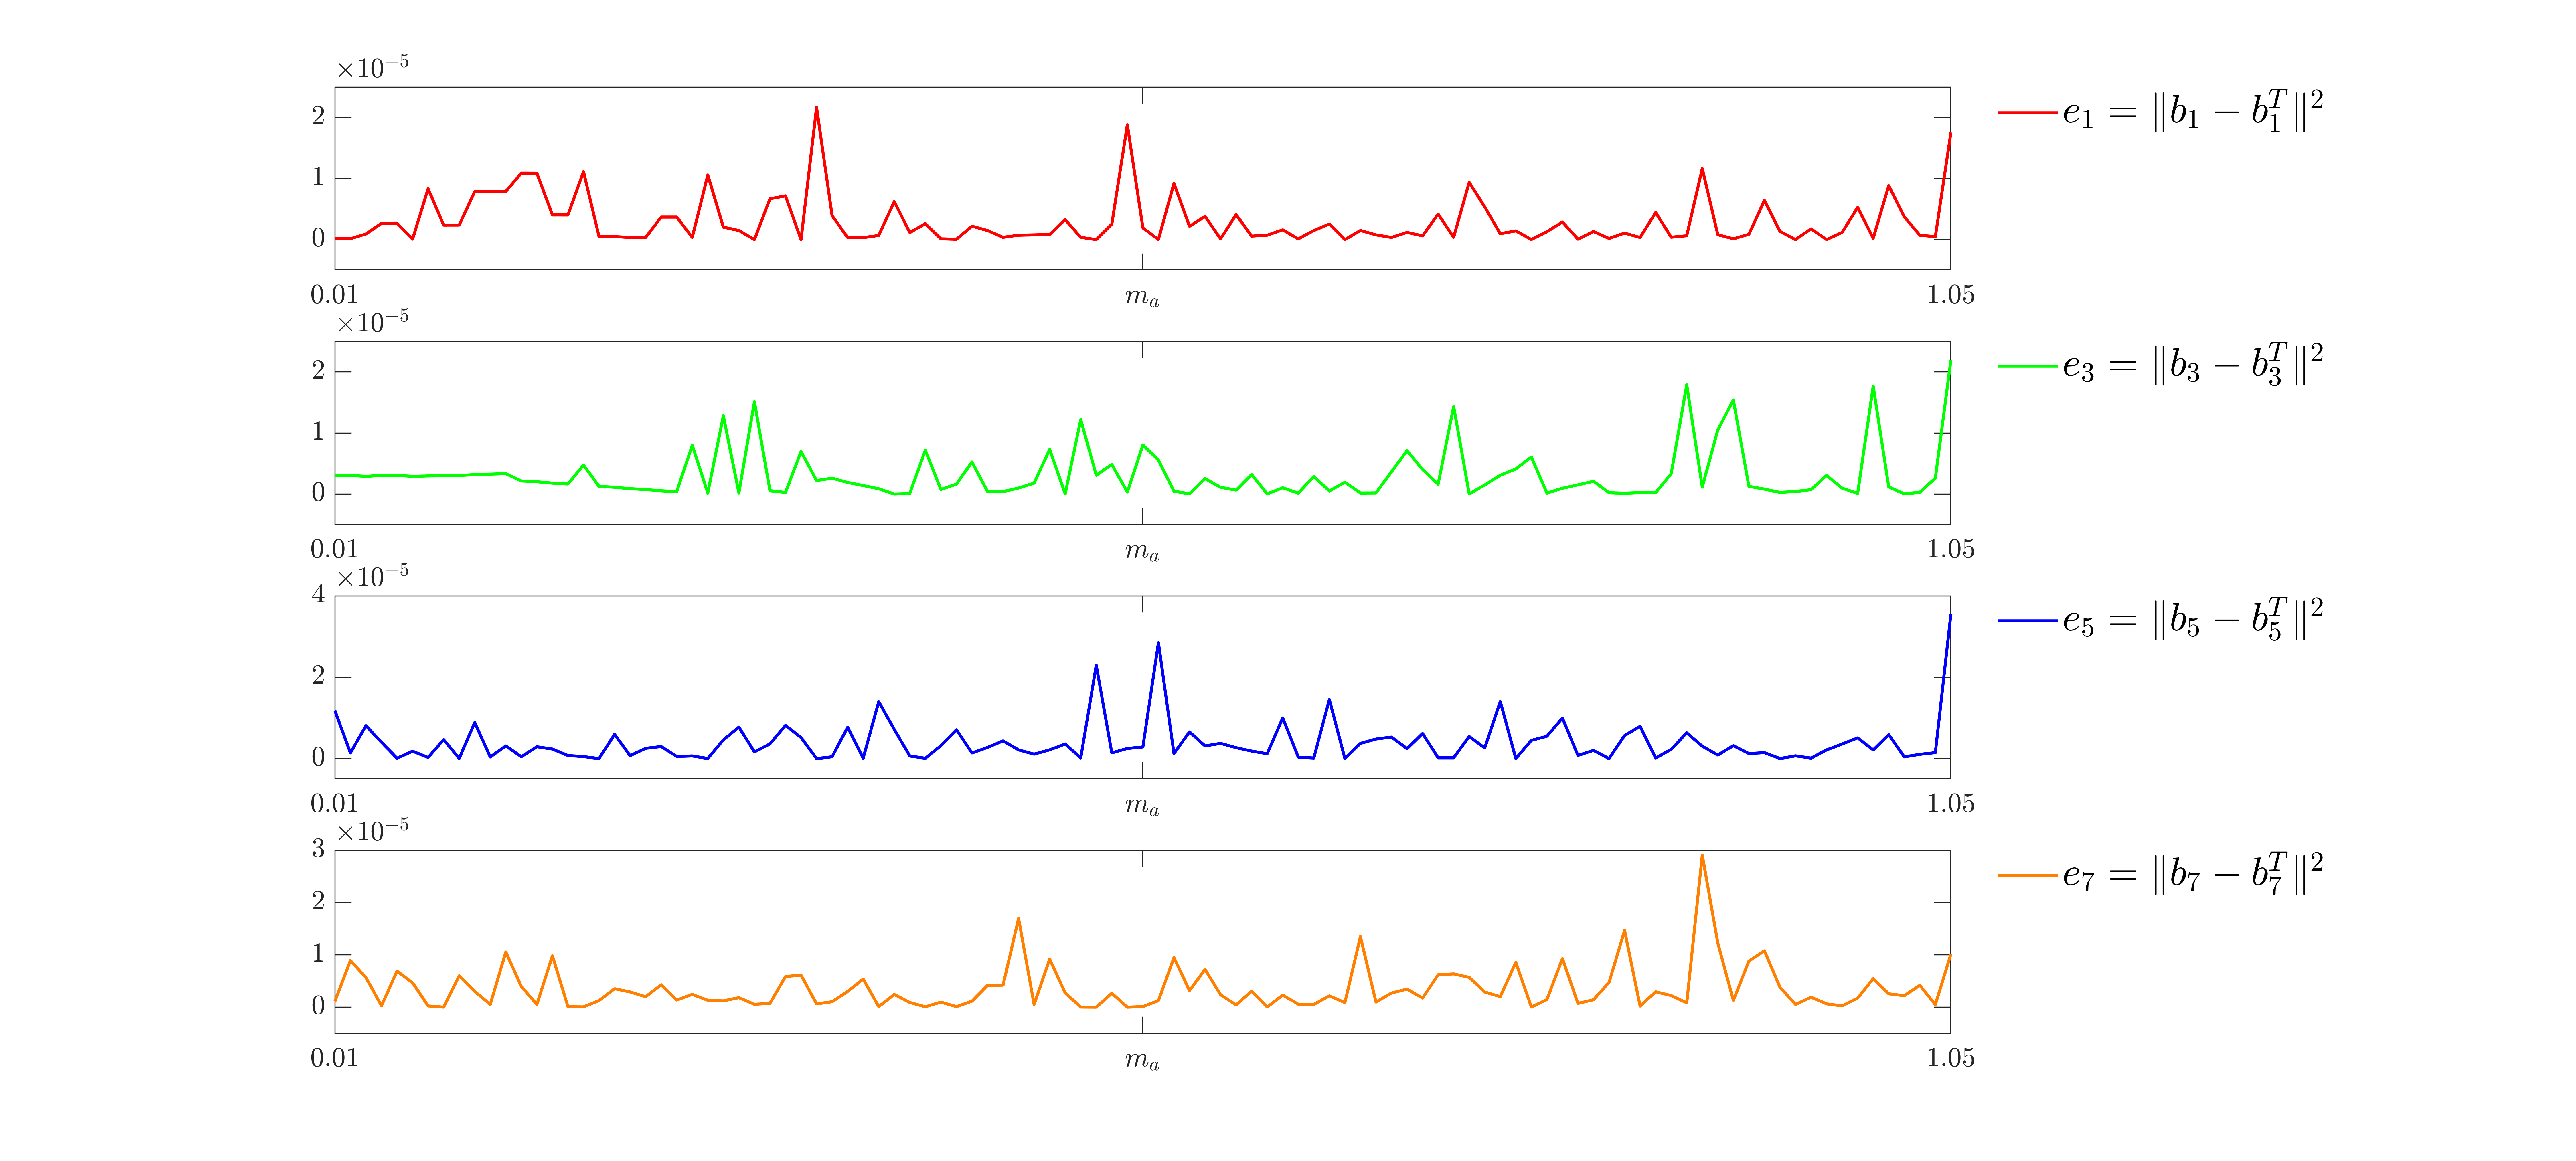
\includegraphics[scale=0.37]{errorElimination}
	\caption{Error $e_{2\ell-1} = \|{\bf{b}}_{2\ell-1}^T-{\bf{b}}_{2\ell-1}\|^2$, $\ell = 1,\ldots,4$.}\label{fig:errorElimination}
\end{figure}

Finally, figure \ref{fig:anglesElimination} shows the behavior of the function $f(\tau)$ with respect to the modulation index and the switching angles. 

\begin{SCfigure}[0.45][h]
	\centering 
	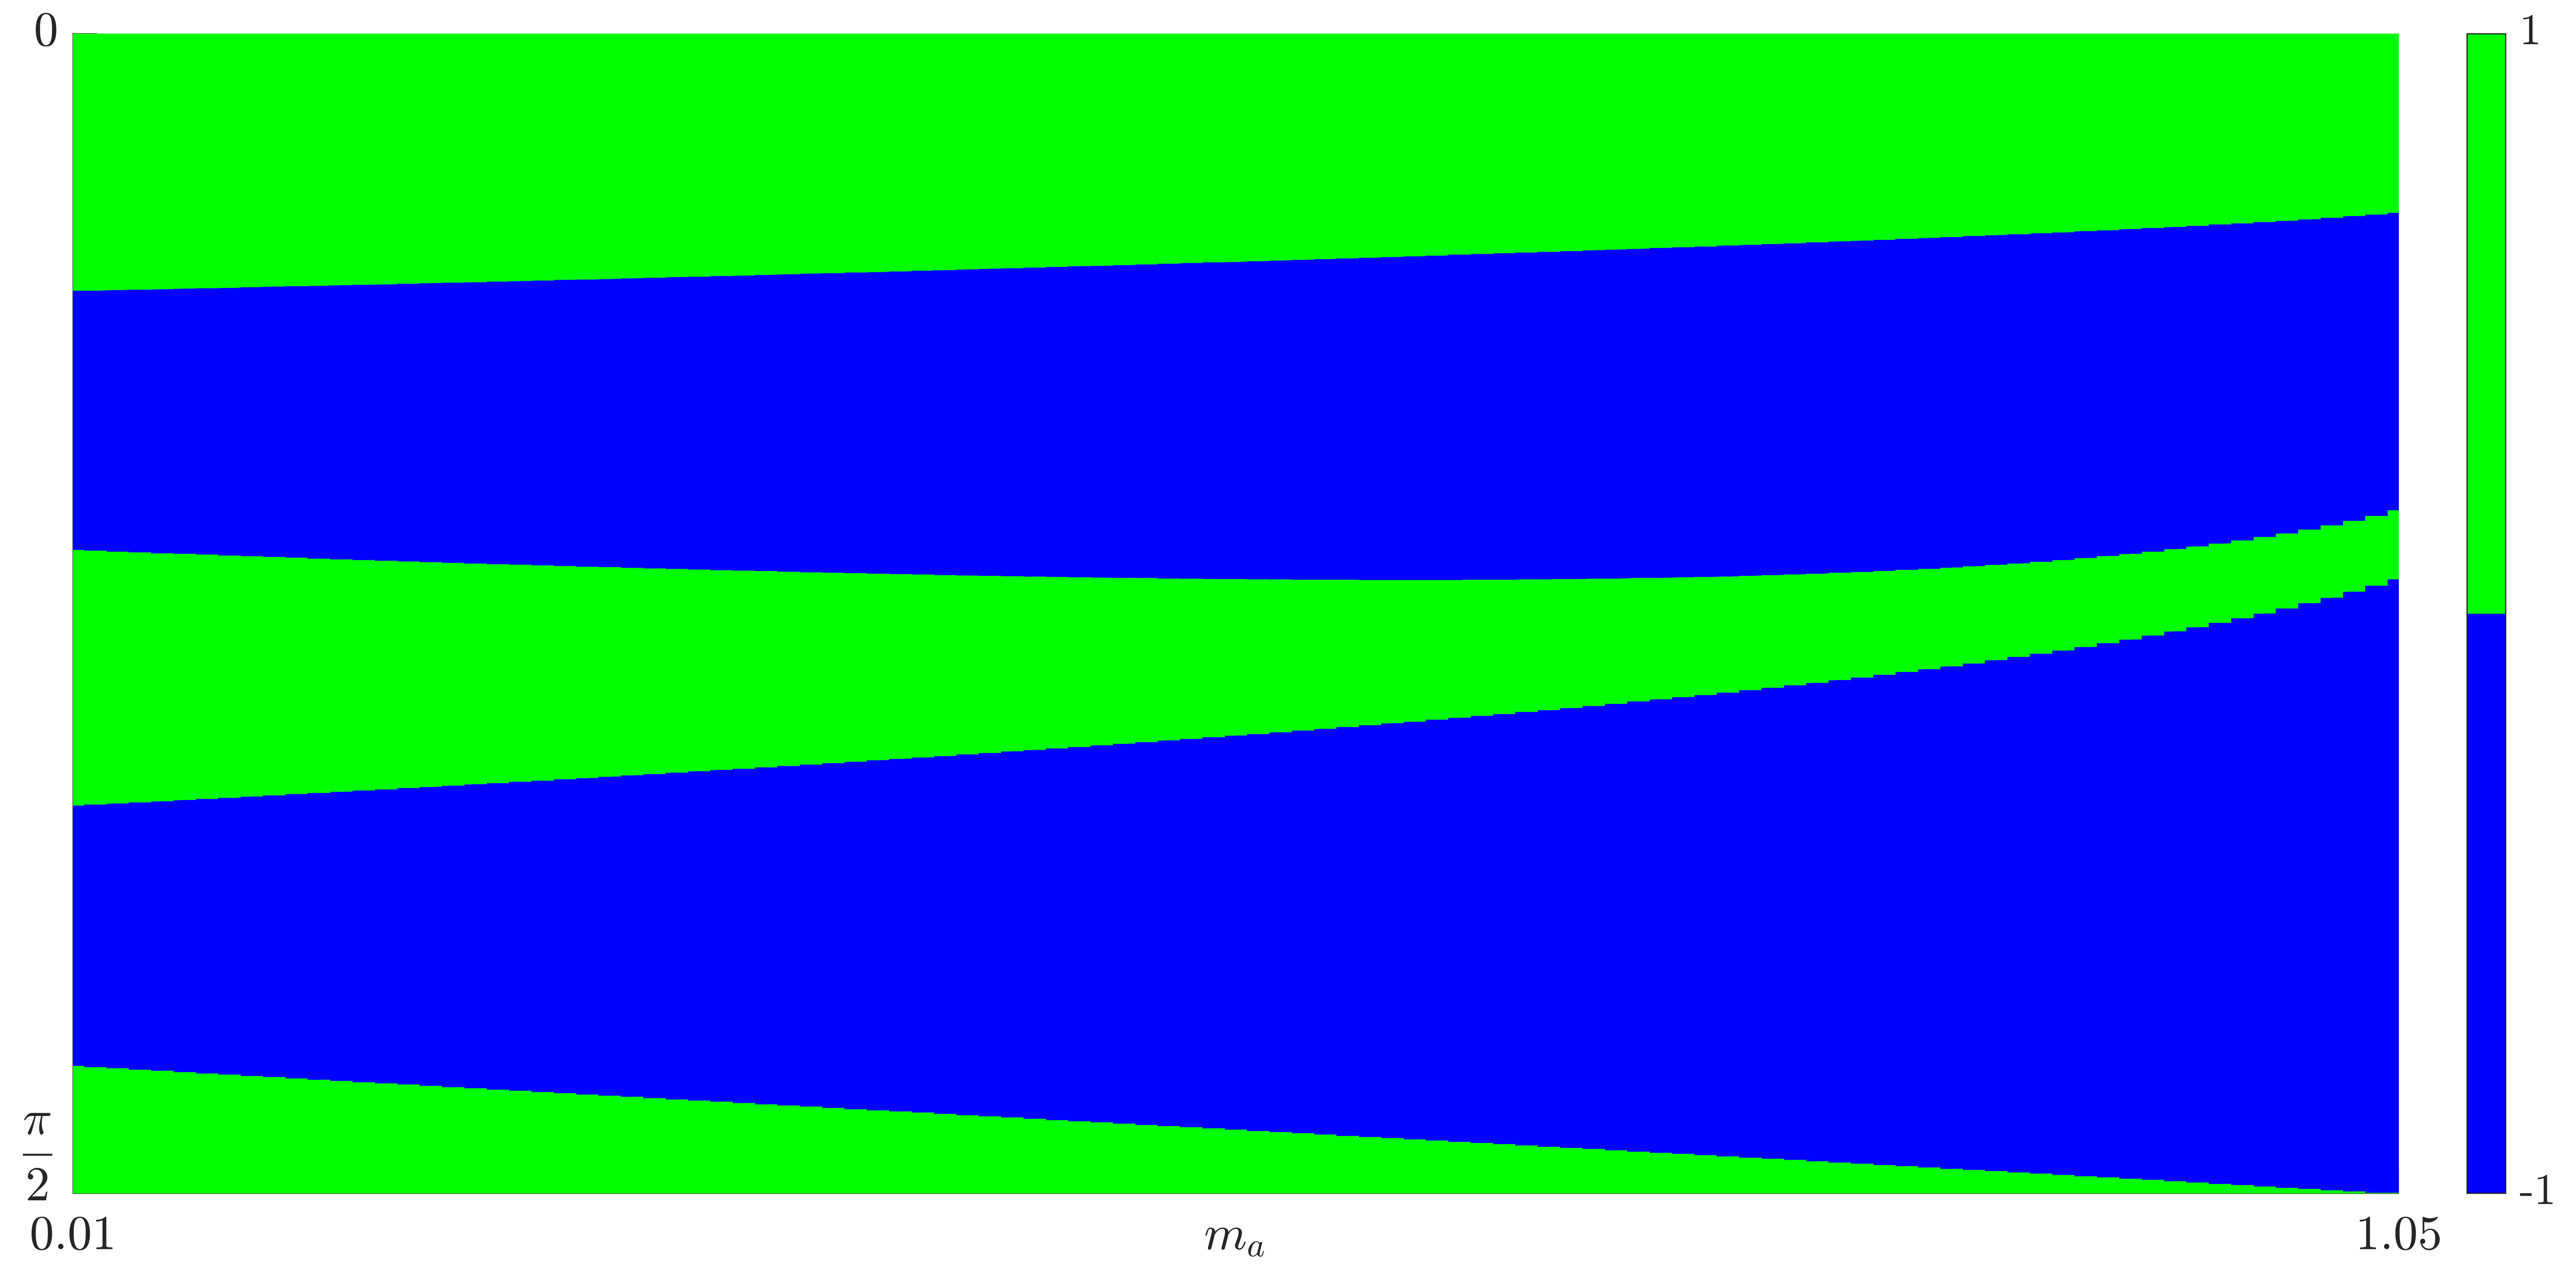
\includegraphics[scale=0.25]{anglesElimination}
	\caption{Behavior of the function $f(\tau)$ for the Selective harmonic Elimination problem with respect to the modulation index (horizontal axis) and the switching angles (vertical axis). The blue region indicates when $f$ takes the value $-1$, while in the green region $f$ takes the value $1$.}\label{fig:anglesElimination}
\end{SCfigure}

\subsection{Selective Harmonic Modulation}

We now consider the Selective Harmonic Elimination problem, in which we want the Fourier coefficients $(b_1,b_3,b_5,b_7)$ to match the target 
\begin{align*}
	(b_1^T,b_3^T,b_5^T,b_7^T) = (0.5m_a,0.05,0,0), \quad m_a\in (0.01,1.12).	
\end{align*}
As before, we considered a $112$-points discretization of the interval $(0.01,1.12)$, 
\begin{align*}
	0.01 = m_{a,1}< m_{a,2} < \ldots < m_{a,i} < m_{a,i+1} < \ldots < m_{a,112} = 1.12
\end{align*}
with $m_{a,i} = 0.01 + (i-1)\Delta m_a$, $i=1,\ldots,112$, $\Delta m_a=10^{-2}$. For each value of $m_{a,i}$, we computed the corresponding vector of target Fourier coefficients
\begin{align*}
	&{\bf{b}}^T_1 =(b_{1,1}^T,b_{1,2}^T,b_{1,3}^T,\ldots, b_{1,112}^T) = 0.5(m_{a,1},m_{a,2},m_{a,3},\ldots,m_{a,112})\in\mathbb{R}^{112},
	\\
	&{\bf{b}}^T_3 =(b_{3,1}^T,b_{3,2}^T,b_{3,3}^T,\ldots, b_{3,112}^T) = (0.05,0.05,0.05,\ldots,0.05)\in\mathbb{R}^{112},
	\\
	&{\bf{b}}^T_5 =(b_{5,1}^T,b_{5,2}^T,b_{5,3}^T,\ldots, b_{5,112}^T) = (0,0,0,\ldots,0)\in\mathbb{R}^{112},
	\\
	&{\bf{b}}^T_7 =(b_{7,1}^T,b_{7,2}^T,b_{7,3}^T,\ldots, b_{7,112}^T) = (0,0,0,\ldots,0)\in\mathbb{R}^{112},
\end{align*}
and used these values to obtain the four coefficients 
\begin{align*}
	s_1 = s_1(b_{1,i}^T), \quad s_3 = s_3(b_{1,i}^T,b_{3,i}^T), \quad s_5 = s_5(b_{1,i}^T,b_{3,i}^T,b_{5,i}^T), \quad s_7 = s_7(b_{1,i}^T,b_{3,i}^T,b_{5,i}^T,b_{7,i}^T), \quad i = 1,\ldots, 112,
\end{align*}
following the procedure presented in Appendix \ref{sec:appendix1}.

We then solved again the corresponding algebraic system \eqref{eq:algebraicEqBkExample} through the procedure presented in Appendix \ref{sec:appendix2}, obtaining the switching angles
\begin{align*}
	&{\bm{\alpha}}_1 =(\alpha_{1,1},\alpha_{1,2},\alpha_{1,3},\ldots,\alpha_{1,112}) \in\mathbb{R}^{112},
	\\
	&{\bm{\alpha}}_2 =(\alpha_{2,1},\alpha_{2,2},\alpha_{2,3},\ldots,\alpha_{2,112}) \in\mathbb{R}^{112},
	\\
	&{\bm{\alpha}}_3 =(\alpha_{3,1},\alpha_{3,2},\alpha_{3,3},\ldots,\alpha_{3,112}) \in\mathbb{R}^{112},
	\\
	&{\bm{\alpha}}_4 =(\alpha_{4,1},\alpha_{4,2},\alpha_{4,3},\ldots,\alpha_{4,112}) \in\mathbb{R}^{112},
\end{align*}

Finally, with these angles we built the function $f(\tau)$ and we employed the formula \eqref{eq:FourCoeffInt} to obtain the Fourier coefficients 
\begin{align*}
	&{\bm{b}}_1 =(b_{1,1},b_{1,2},b_{1,3},\ldots,b_{1,112}) \in\mathbb{R}^{112},
	\\
	&{\bm{b}}_3 =(b_{3,1},b_{3,2},b_{3,3},\ldots,b_{3,112}) \in\mathbb{R}^{112},
	\\
	&{\bm{b}}_5 =(b_{5,1},b_{5,2},b_{5,3},\ldots,b_{5,112}) \in\mathbb{R}^{112},
	\\
	&{\bm{b}}_7 =(b_{7,1},b_{7,2},b_{7,3},\ldots,b_{7,112}) \in\mathbb{R}^{112},
\end{align*}
and we compared them with the target vectors ${\bf{b}}_{2\ell-1}^T$, $\ell=1,\ldots,4$, by computing the quadratic error
\begin{align*}
	e_{2\ell-1} = \|{\bf{b}}_{2\ell-1}^T-{\bf{b}}_{2\ell-1}\|^2.
\end{align*}
These errors are displayed in Figure \ref{fig:errorModulation}.

\begin{figure}[h]
	\centering
	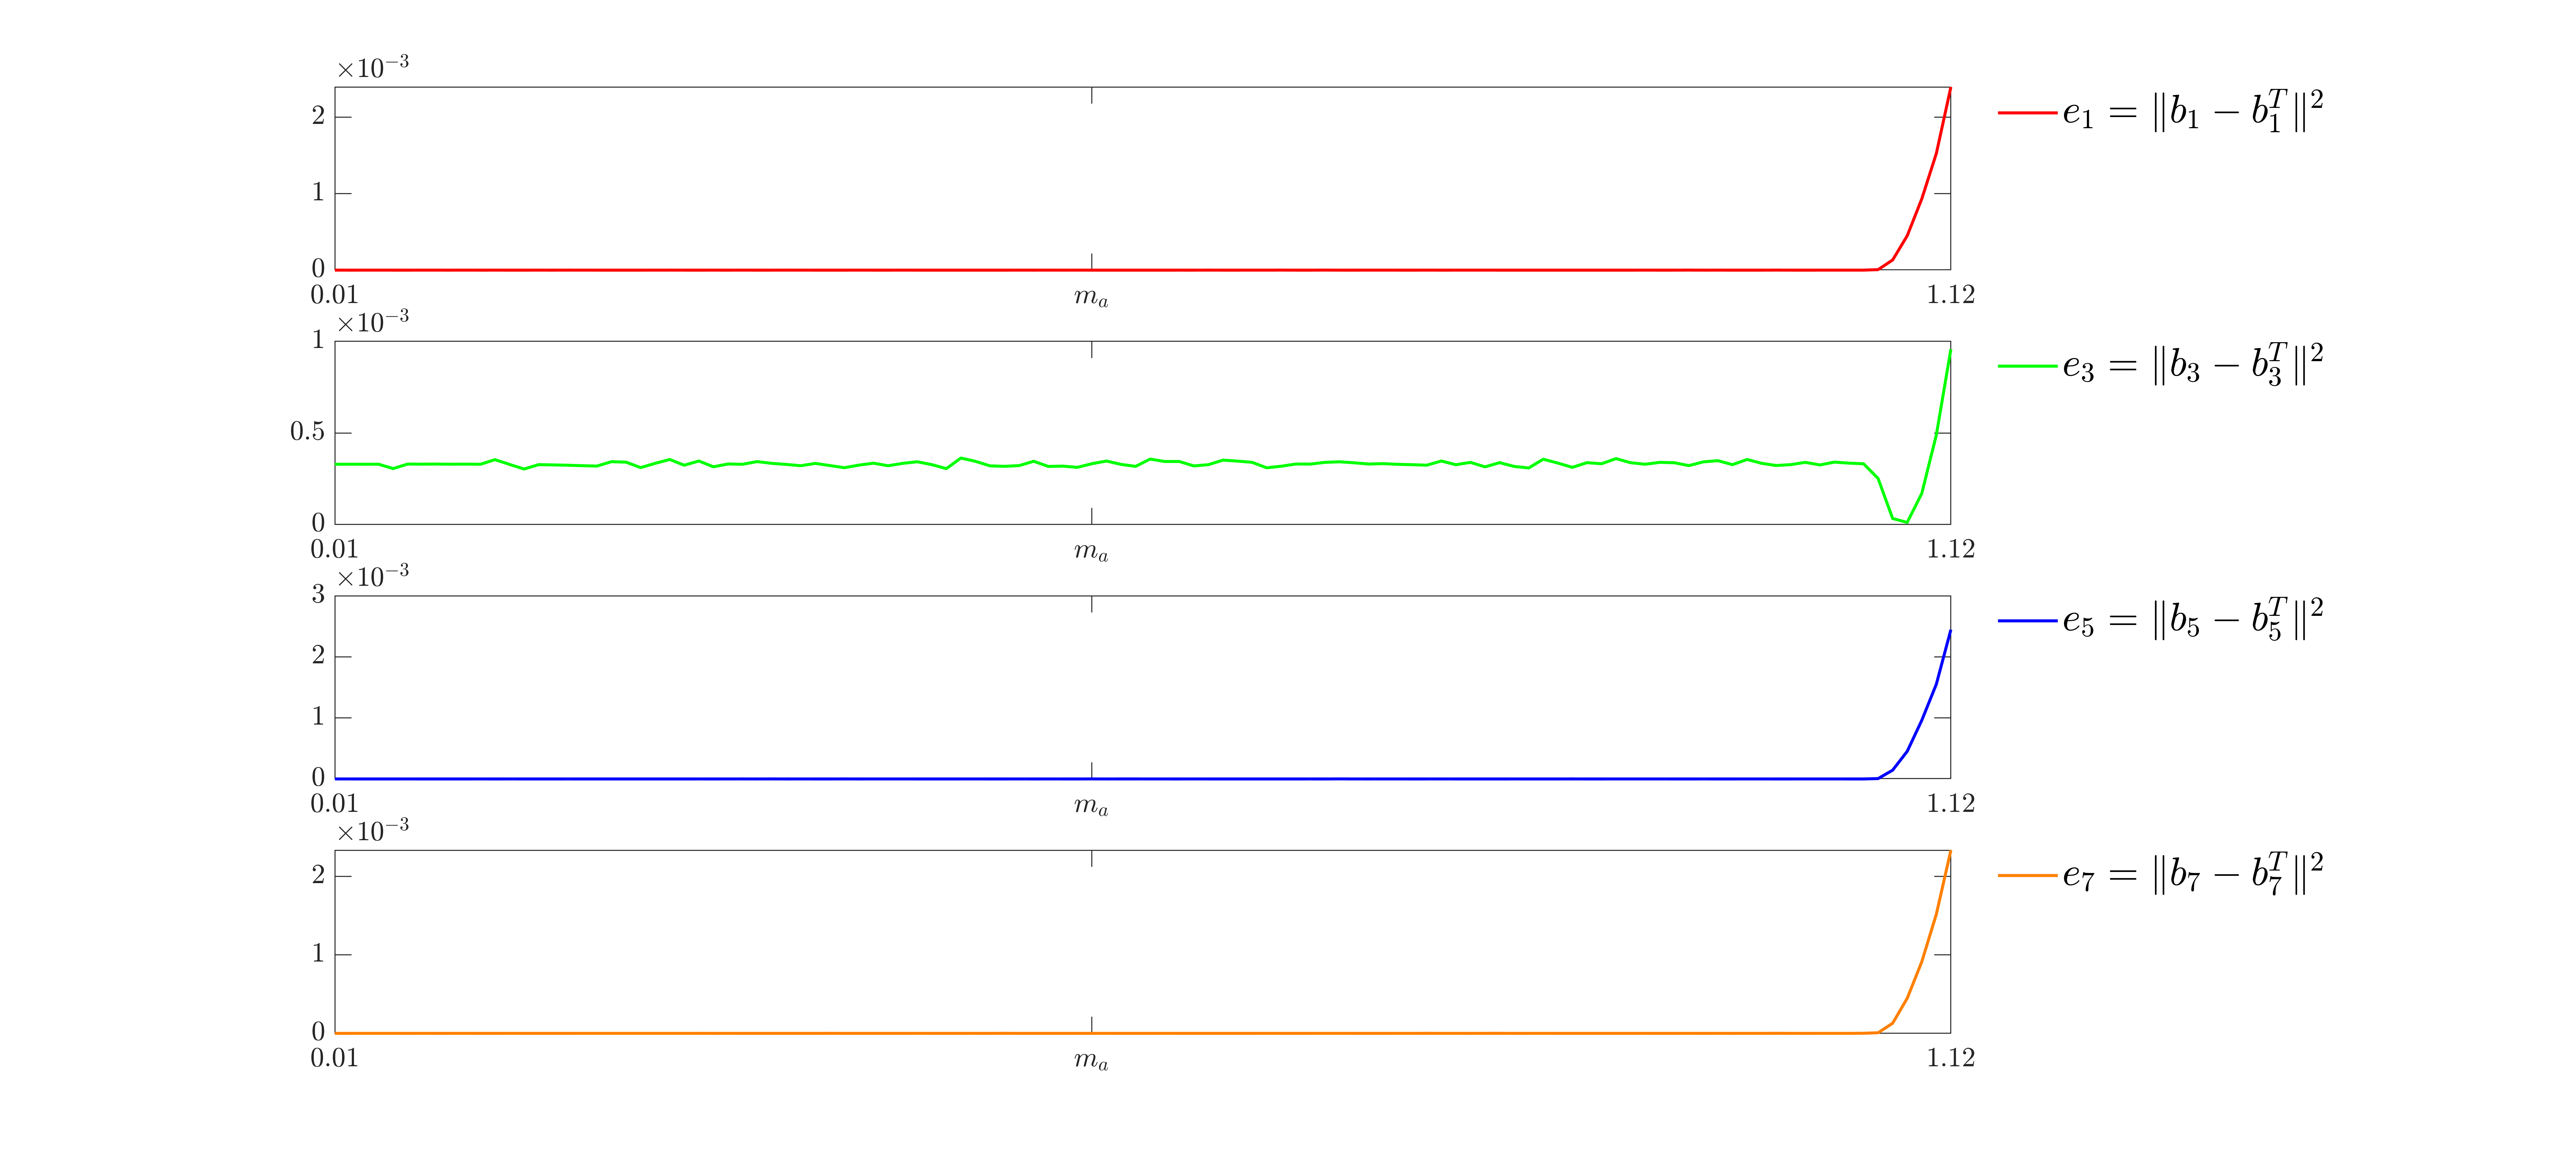
\includegraphics[scale=0.3]{errorModulation}
	\caption{Error $e_{2\ell-1} = \|{\bf{b}}_{2\ell-1}^T-{\bf{b}}_{2\ell-1}\|^2$, $\ell = 1,\ldots,4$.}\label{fig:errorModulation}
\end{figure}

Finally, figure \ref{fig:anglesModulation} shows the behavior of the function $f(\tau)$ with respect to the modulation index and the switching angles. 

\begin{SCfigure}[0.45][h]
	\centering 
	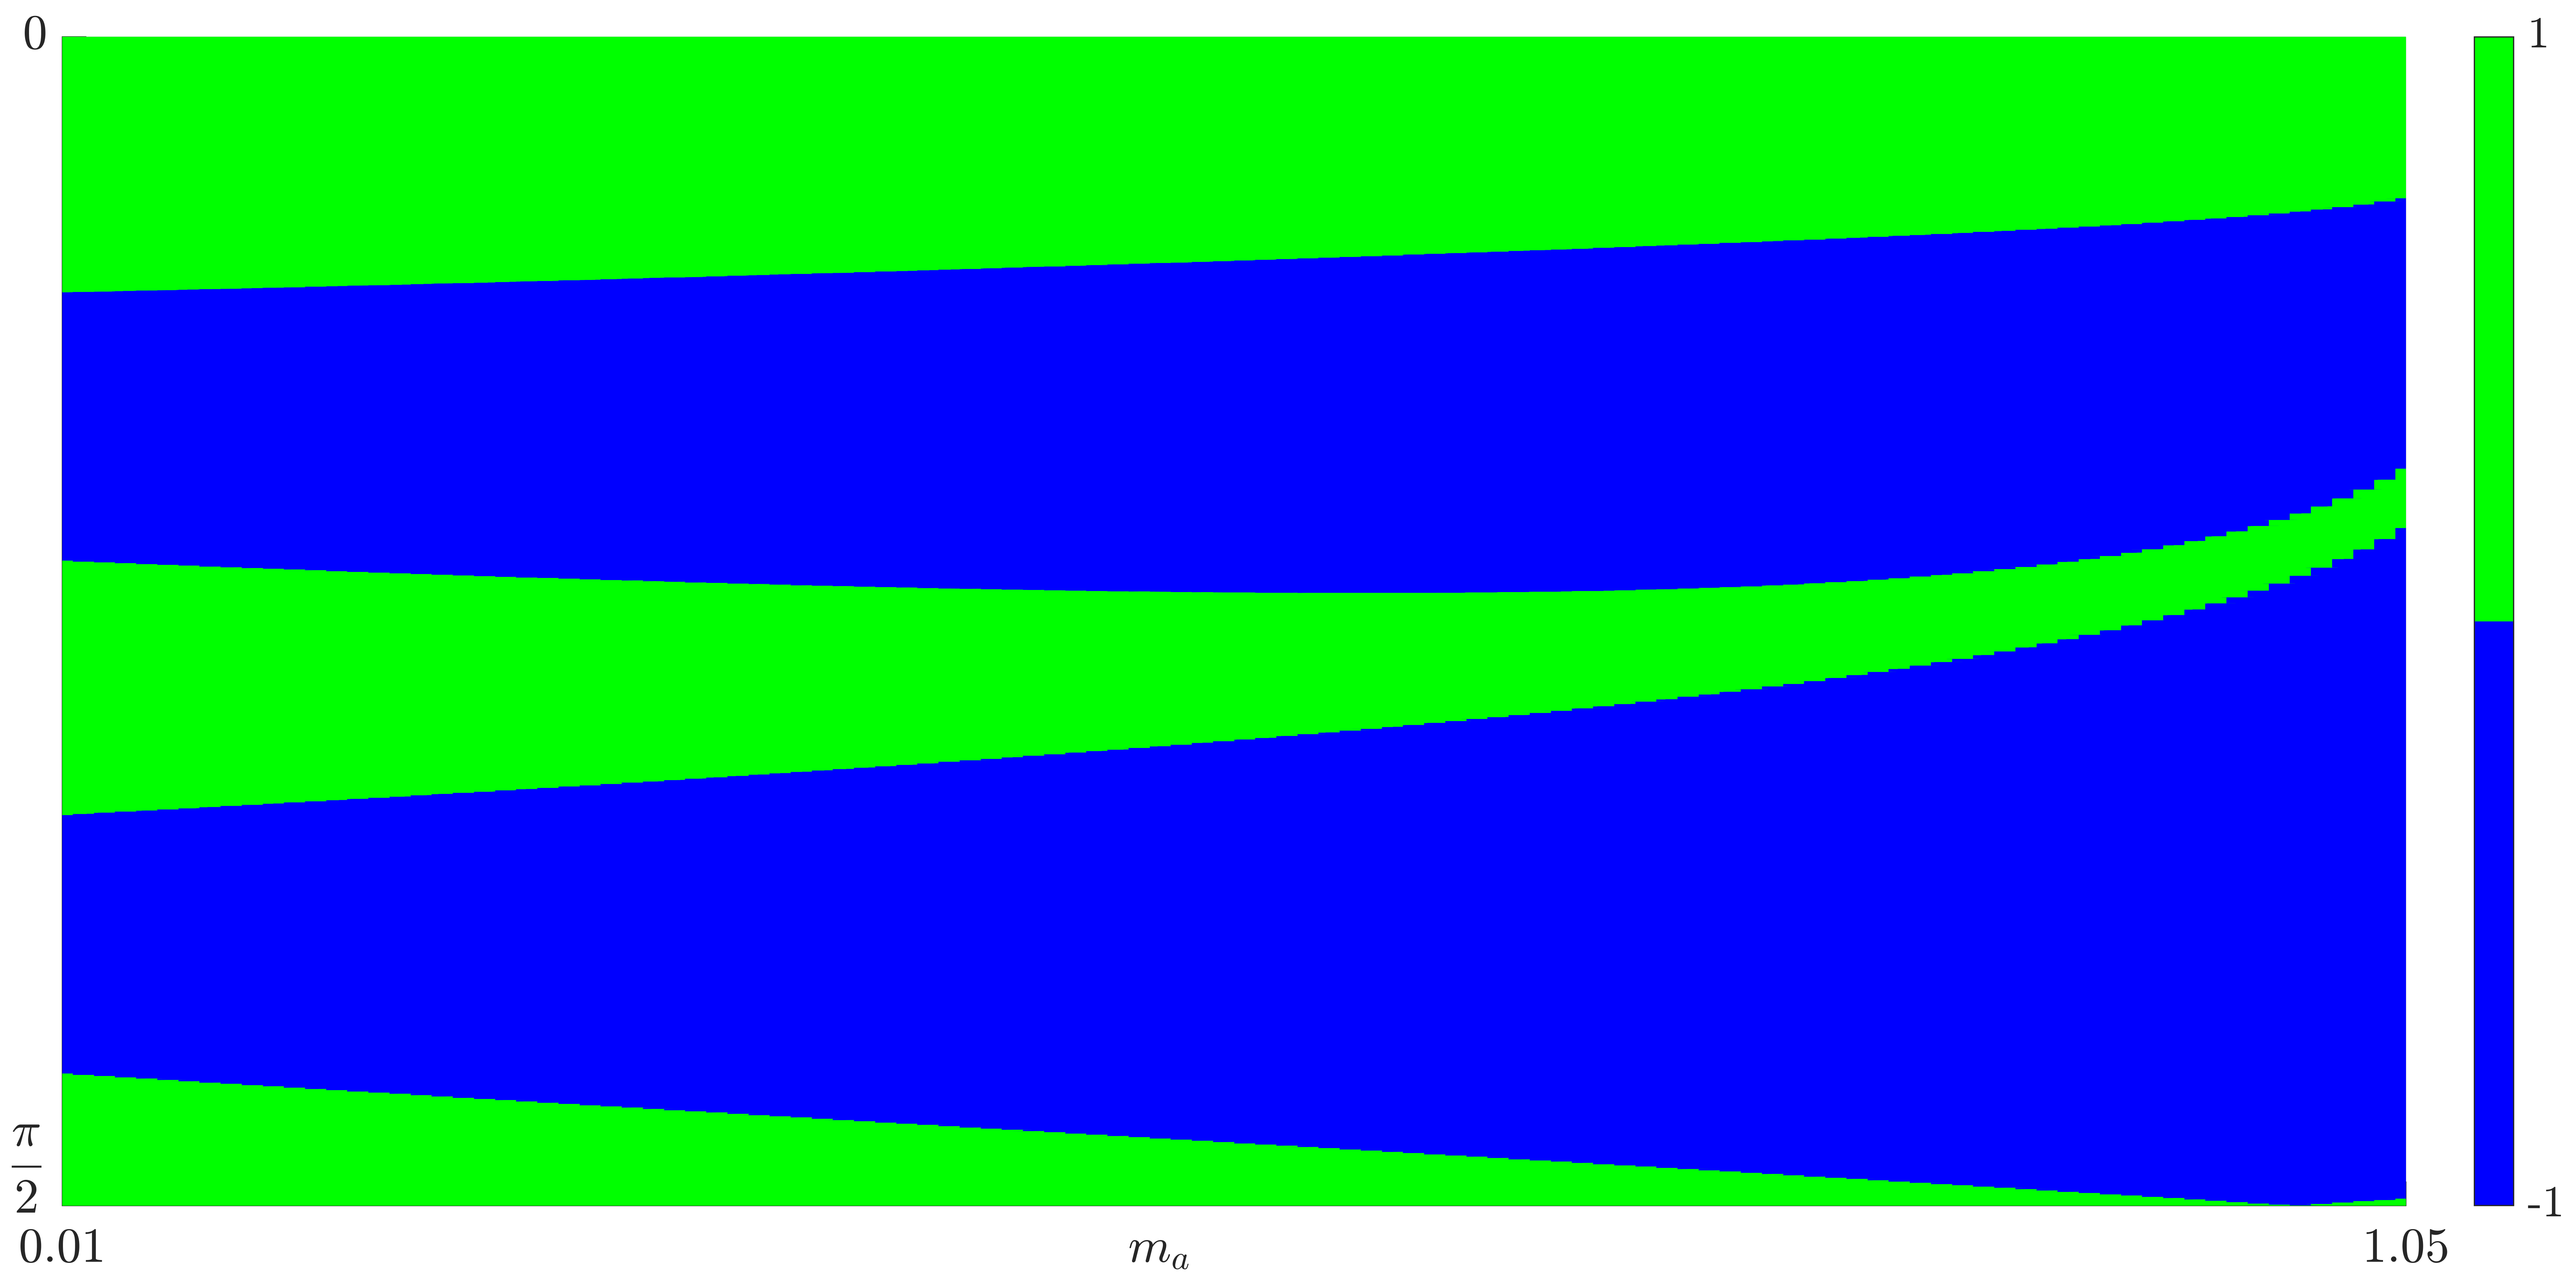
\includegraphics[scale=0.25]{anglesModulation}
	\caption{Behavior of the function $f(\tau)$ for the Selective Harmonic Modulation problem with respect to the modulation index (horizontal axis) and the switching angles (vertical axis). The blue region indicates when $f$ takes the value $-1$, while in the green region $f$ takes the value $1$.}\label{fig:anglesModulation}
\end{SCfigure}


\appendix{
\section{Transformation of \eqref{eq:transcEqBkSquare} in a set of algebraic equations}\label{sec:appendix1}

As we said, in order to solve system \eqref{eq:transcEqBkSquare}, we shall transform the transcendental equations in algebraic ones. The procedure to apply summarizes as follows:

\paragraph{Step 1.} We apply the changes of variables \eqref{eq:changeVariables} to the first equation in \eqref{eq:transcEqBkSquare}, obtaining
\begin{align*}
	x_1 + x_2 + \ldots + x_n = \frac 12 + \frac{\pi b_1}{8V_{dc}}=:s_1.
\end{align*}

\paragraph{Step 2.} By considering the Chebyshev polynomials 
\begin{align*}
	T_0(x) = 1, \quad T_1(x) = x, \quad T_{j+1}(x) = 2xT_j(x)-T_{j-1}(x)
\end{align*}
and their trigonometric definition 
\begin{align*}
	T_j(x) = \cos(j\mbox{arccos}(x)),\quad |x|\leq 1,
\end{align*}
we have for all $i=1,2\ldots,n$
\begin{align*}
	&T_0(\cos(\alpha_i)) = 1,
	\\
	&T_1(\cos(\alpha_i)) = \cos(\alpha_i),
	\\
	&T_2(\cos(\alpha_i)) = \cos(2\alpha_i) = 2\cos(\alpha_i)T_1(\cos(\alpha_i)) -T_0(\cos(\alpha_i)) = 2\cos^2(\alpha_i)-1,
	\\
	&T_3(\cos(\alpha_i)) = \cos(3\alpha_i) = 2\cos(\alpha_i)T_2(\cos(\alpha_i)) -T_1(\cos(\alpha_i)) = 4\cos^3(\alpha_i)-3\cos(\alpha_i).
\end{align*}
Hence, from the second equation in \eqref{eq:transcEqBkSquare} we get
\begin{align*}
	\frac 12 + \frac{3\pi b_3}{8V_{dc}} & = \sum_{i=1}^n (-1)^{i+1} \cos (3\alpha_i) = 4\sum_{i=1}^n (-1)^{i+1} \cos^3(\alpha_i) - 3\sum_{i=1}^n (-1)^{i+1} \cos(\alpha_i).
\end{align*}
Using again the change of variables \eqref{eq:changeVariables}, and noticing that 
\begin{align*}
	x_i^3 = (-1)^{3i+3}\cos^3(\alpha_i) = (-1)^{i+1}\cos^3(\alpha_i), \quad i=1,2,\ldots,n,
\end{align*} 
we obtain
\begin{align*}
	\frac 12 + \frac{3\pi b_3}{8V_{dc}} & = 4(x_1^3 + x_2^3 + \ldots + x_n^3) - 3(x_1 + x_2 + \ldots + x_n) = 4(x_1^3 + x_2^3 + \ldots + x_n^3) - 3s_1.
\end{align*}
This yields
\begin{align*}
	x_1^3 + x_2^3 + \ldots + x_n^3 = \frac 14\left(\frac 12 + \frac{3\pi b_3}{4V_{dc}} + 3s_1\right) = \frac 12\left(1 + \frac 34\frac{\pi b_3}{4V_{dc}} + \frac 34\frac{\pi b_1}{4V_{dc}}\right):=s_3.
\end{align*}

\paragraph{Step 3.} By employing once again the Chebyshev polynomials, we can easily compute $\cos(5\alpha_i)$
\begin{align*}
	T_5(\cos(\alpha_i)) = \cos(5\alpha_i) = 16\cos^5(\alpha_i)-20\cos^3(\alpha_i)+5\cos(\alpha_i).
\end{align*}
Hence, from the third equation in \eqref{eq:transcEqBkSquare} we get
\begin{align*}
	\frac 12 + \frac{5\pi b_5}{8V_{dc}} & = \sum_{i=1}^n (-1)^{i+1} \cos (5\alpha_i) 
	\\
	&= 16\sum_{i=1}^n (-1)^{i+1} \cos^5(\alpha_i) - 20\sum_{i=1}^n (-1)^{i+1} \cos^3(\alpha_i) + 5\sum_{i=1}^n (-1)^{i+1} \cos(\alpha_i).
\end{align*}
Using again the change of variables \eqref{eq:changeVariables}, and noticing that 
\begin{align*}
	x_i^5 = (-1)^{5i+5}\cos^5(\alpha_i) = (-1)^{i+1}\cos^5(\alpha_i), \quad i=1,2,\ldots,n,
\end{align*} 
we obtain
\begin{align*}
	\frac 12 + \frac{5\pi b_5}{8V_{dc}} & = 16(x_1^5 + x_2^5 + \ldots + x_n^5) -20(x_1^3 + x_2^3 + \ldots + x_n^3) + 5(x_1 + x_2 + \ldots + x_n) 
	\\
	&= 16(x_1^5 + x_2^5 + \ldots + x_n^5) - 20s_3 + 5s_1.
\end{align*}
This yields
\begin{align*}
	x_1^5 + x_2^5 + \ldots + x_n^5 = \frac{1}{16}\left(\frac 12 + \frac{5\pi b_5}{8V_{dc}} + 20s_3 - 5s_1\right) = \frac{1}{16}\left(8 + \frac 52\frac{\pi b_5}{4V_{dc}} + \frac{15}{2} \frac{\pi b_3}{4V_{dc}} - \frac 52\frac{\pi b_1}{4V_{dc}}\right):=s_5.
\end{align*}

\paragraph{Step 4.} By iterating the above procedure we get the general algebraic equation
\begin{align}
	x_1^{2n-1} + x_2^{2n-1} + \ldots + x_n^{2n-1} = s_{2n-1},
\end{align}
where the coefficients $s_{2n-1}$ are obtained through the recursive algorithm
\begin{align}\label{eq:s_iAlgo}
	&\left. T_1(x)\right|_{x=s_1} = s_1 = \frac 12 +\frac{\pi b_1}{8V_{dc}}, \notag
	\\
	&\left. T_{2n-1}(x)\right|_{x^{2n-1}=s_{2n-1}} = \frac 12 +\frac{(2n-1)\pi b_{2n-1}}{8V_{dc}}, \quad n\geq 2.
\end{align}

The procedure \eqref{eq:s_iAlgo} to compute the coefficients $\{s_{2\ell-1}\}_{\ell=1}^n$ is implemented through the Matlab functions presented in Algorithms \ref{alg:coefficients_s} and \ref{alg:chebyshev}.

\begin{algorithm}
	\caption{Computation of the coefficients $\{s_{2\ell-1}\}_{\ell=1}^n$ in \eqref{eq:algebraicEqBkSquare}} \label{alg:coefficients_s}
	\begin{lstlisting}[style=Matlab-editor, basicstyle=\mlttfamily\footnotesize]
		function S = coeffSHE(b,Vdc)
		
		n = length(b);
		s = 0.5 + (pi*b(1)/(8*Vdc));
		s = [0 s 0];
		rhs = 0.5 + (1/(4*Vdc))*[1:2:2*n].*b; 
		j = 2;
		
		for i = 3:2:2*n
			c = ChebPoly(i);
			aux = (rhs(j)-c(2:end)*s')/c(1);
			s = [0 aux s];
			j = j+1;
		end
		
		s = fliplr(double(s));
		S = s(s~=0);
	\end{lstlisting}
\end{algorithm}

\begin{algorithm}
	\caption{Coefficients of the $n$-th Chebyshev polynomial} \label{alg:chebyshev}
	\begin{lstlisting}[style=Matlab-editor, basicstyle=\mlttfamily\footnotesize]
		function c = ChebPoly(n)
		
		PolyOrder = 1:2:2*n-1;
		L = length(PolyOrder);
		C = zeros(L+1,L+1);
		
		C(1,end) = 1;
		C(2,end-1) = 1;
		
		for i = 3:L+1
			aux = 2*circshift(C(i-1,:),-1);
			C(i,:) = aux-C(i-2,:);
		end
		
		c = C(end,:);
	\end{lstlisting}
\end{algorithm}

\section{Resolution of the algebraic equations}\label{sec:appendix2}

Let us now discuss the resolution of \eqref{eq:algebraicEqBkSquare}. To this end, let us introduce the function
\begin{align}\label{eq:FunctionG}
	G(x) = \exp\left(-\sum_{\underset{\ell\,odd}{\ell\geq 1}}\left(\sum_{i=1}^n \frac{x_i^\ell}{\ell}\right)x^{-\ell}\right).
\end{align}
Then, according to \cite[Theorem 1]{chudnovsky1999solution}, the solution $\{x_i\}_{i=1}^n$ of \eqref{eq:algebraicEqBkSquare} is given by the roots of the numerator 
\begin{align*}
	p(x) = \prod_{i=1}^n (x-x_i) = \sum_{m=0}^n p_mx^{n-m}.
\end{align*}
in the Pad\'e approximation of order $(n,n)$ of $G$:
\begin{align}\label{eq:pade}
	G(x) = \frac{p(x)}{q(x)},
\end{align}
with $p(x)$ and $q(x)$ two polynomials of degree $n$. Hence, to solve \eqref{eq:algebraicEqBkSquare} we need to determine $p(x)$ and compute its roots. Moreover, let us recall that the Pad\'e approximation of a function is unique. Hence, also the solution $\{x_i\}_{i=1}^n$ of \eqref{eq:algebraicEqBkSquare} will be unique.

Notice that $G(-x) = (G(x))^{-1}$. Then, the Pad\'e approximant $q(x)$ has the property $q(x) = (-1)^np(-x)$ and, from \eqref{eq:pade}, we easily obtain the identity
\begin{align}\label{eq:p}
	p(x) = (-1)^np(-x)G(x).
\end{align}
Let us now introduce the functions
\begin{align}\label{eq:vDef}
	v(x) = -2\sum_{\underset{\ell\; odd}{\ell\geq 1}}\left(\sum_{i=1}^n \frac{x_i^\ell}{\ell}\right) x^\ell, \quad\quad g(x) = \exp\big(v(x)\big).
\end{align}
Then, $G(x) = g(1/x)$ and \eqref{eq:p} can be rewritten as
\begin{align}\label{eq:pExpansion}
	p(x) = (-1)^np(-x)g\left(\frac 1x\right).
\end{align}
We can now use \eqref{eq:pExpansion} to obtain explicitly the coefficients $\{p_m\}_{m=0}^n$ through the following procedure.

\paragraph{Step 1.} First of all, let us introduce the series expansion of $v(x)$:
\begin{align*}
	v(x) = \sum_{\ell\geq 0} v_\ell x^\ell.
\end{align*} 
Comparing this with \eqref{eq:vDef}	we get
\begin{align*}
	v(x) = -2\sum_{\underset{\ell\; odd}{\ell\geq 1}}\left(\sum_{i=1}^n \frac{x_i^\ell}{\ell}\right) x^\ell = \sum_{\ell\geq 0} v_\ell x^\ell
\end{align*}
and, equating the coefficients of the same order, we have
\begin{align}\label{eq:coefficientsV}
	\begin{cases}
		\displaystyle v_\ell=-2\sum_{i=1}^n\frac{x_i^\ell}{\ell}, &\mbox{ for } \ell \mbox{ odd}
		\\
		v_\ell=0, &\mbox{ for } \ell \mbox{ even}.
	\end{cases}
\end{align}
Notice that, according to \eqref{eq:algebraicEqBkSquare}, we have
\begin{align*}
	\sum_{i=1}^n x_i^\ell = s_\ell \quad\mbox{ for }\ell = 1,3,5,\ldots 2n-1.
\end{align*}
Hence, from \eqref{eq:coefficientsV} we can compute the coefficients $v_\ell$ up to $\ell = 2n$ as
\begin{align}\label{eq:coefficientsVexpl}
	\begin{cases}
		\displaystyle v_\ell=-\frac{2s_\ell}{\ell}, &\mbox{ for } \ell = 1,\ldots, 2n,\quad\ell \mbox{ odd}
		\\
		v_\ell=0, &\mbox{ for } \ell \mbox{ even}.
	\end{cases}
\end{align}

This is done with the Matlab function presented in Algorithm \ref{alg:coefficients_v}. Nevertheless, for $\ell\geq 2n+1$, we can only know the even coefficients (which are all zero) while the odd coefficients cannot be computed.
\begin{algorithm}
	\caption{Computation of the coefficients $\{v_\ell\}_{\ell=1}^{2n}$ using \eqref{eq:coefficientsVexpl}} \label{alg:coefficients_v}
	\begin{lstlisting}[style=Matlab-editor, basicstyle=\mlttfamily\footnotesize]
		function v = coefficients_v(s)
		
		[lMa,n] = size(s);
		
		% The i-th row of the matrix v contains the 2n coefficients v_i
		% corresponding to the i-th value of the modulation index
		
		v = zeros(lMa,2*n);
		
		for l = 1:n
			v(:,2*l-1) = -(2/(2*l-1))*s(:,l);
		end
	\end{lstlisting}
\end{algorithm}

\paragraph{Step 2.} Let us now introduce the series expansion of $g(x)$
\begin{align*}
	g(x) = \sum_{\ell\geq 0} g_\ell x^\ell 
\end{align*} 
and notice that, from the expression $g(x) = \exp\big(v(x)\big)$, we obtain
\begin{align*}
	\frac{dg(x)}{dx} = \frac{dv(x)}{dx}g(x).
\end{align*}
Expanding both sides of the identity above, we get
\begin{align*}
	g_1 + 2g_2x + 3g_3x^2 + \ldots &= (v_1 + 2v_2x + 3v_3x^2 + \ldots)(g_0 + g_1x + g_2x^2 + \ldots)
	\\
	&= (v_1g_0) + (2v_2g_0 + v_1g_1)x + (3v_3g_0 + 2v_2g_1 + v_1g_2)x^2 + \ldots 
\end{align*}

By setting $g_0=1$ (which yields $v_0 = \ln(g_0) =0$) and equating the coefficients of the left and right-hand side, we thus find that
\begin{align}\label{eq:coefficientsG}
	g_0 = 1, \quad g_\ell = \sum_{k=1}^\ell \frac k\ell v_kg_{\ell-k} = \sum_{\underset{k\; odd}{k=1}}^\ell \frac k\ell v_kg_{\ell-k} \quad\mbox{ for } \ell\geq 1. 
\end{align}

Recall that \eqref{eq:coefficientsVexpl} allows to obtain the coefficients $\{v_\ell\}_{\ell=1}^{2n}$. Hence, we can use \eqref{eq:coefficientsG} to compute $\{g_\ell\}_{\ell=1}^{2n}$ through the Matlab function presented in Algorithm \ref{alg:coefficients_g}. Nevertheless, also in this case, for $\ell\geq 2n+1$ the coefficients $g_\ell$ cannot be computed.

\begin{algorithm}
	\caption{Computation of the coefficients $\{g_\ell\}_{\ell=1}^{2n}$ using \eqref{eq:coefficientsG}} \label{alg:coefficients_g}
	\begin{lstlisting}[style=Matlab-editor, basicstyle=\mlttfamily\footnotesize]
		function g = coefficients_g(v)
		
		[lMa,n] = size(v);
		
		% The i-th row of the matrix g contains the 2n coefficients g_i
		% corresponding to the i-th value of the modulation index
		
		g = zeros(lMa,n+1);
		g(:,1) = 1;
		for l = 2:n+1
			G = 0;		
			for k = 1:l-1
				G = G + (k/(l-1))*v(:,k).*g(:,l-k);
			end		
			g(:,l) = G;
		end
	\end{lstlisting}
\end{algorithm}

\paragraph{Step 3.} From \eqref{eq:pExpansion} we have
\begin{align*}
	p(x) = (-1)^np(-x)g\left(\frac 1x\right) = (-1)^np(-x)\left(g_0 + \frac{g_1}{x} + \frac{g_2}{x^2} + \ldots\right),
\end{align*}
which gives
\begin{align*}
	\sum_{m=0}^n p_m x^{n-m} &= (-1)^n\left(\sum_{m=0}^n p_m (-x)^{n-m}\right)\left(\sum_{m\geq 0} g_m x^{-m}\right) = \left(\sum_{m=0}^n (-1)^{2n-m} p_m x^{n-m}\right)\left(\sum_{m\geq 0} g_m x^{-m}\right)
	\\
	&= \left(\sum_{m=0}^n (-1)^m p_m x^{n-m}\right)\left(\sum_{m\geq 0} g_m x^{-m}\right).
\end{align*}

By developing the products on the right-hand side of the above identity, and taking into account that $p_0=1=g_0$, we get 
\begin{align*}
	\sum_{m=0}^n p_mx^{n-m} =& \sum_{m\geq 0} g_m x^{n-m} - \sum_{m\geq 0} p_1g_m x^{n-1-m} + \sum_{m\geq 0} p_2g_m x^{n-2-m} + \ldots + (-1)^n \sum_{m\geq 0} p_ng_m x^{-m} 
	\\
	=&\; x^n + g_1x^{n-1} + g_2x^{n-2} + \ldots + g_{n-1}x + g_n + \sum_{m\geq n+1} g_m x^{n-m} 
	\\
	&- p_1x^{n-1} - p_1g_1x^{n-2} - p_1g_2x^{n-3} - \ldots - p_1g_{n-2}x - p_1g_{n-1} - \sum_{m\geq n} p_1g_m x^{n-1-m} 
	\\
	&+ p_2x^{n-2} + p_2g_1x^{n-3} + p_2g_2x^{n-4} + \ldots + p_2g_{n-3}x + p_2g_{n-2} + \sum_{m\geq n-1} p_2g_m x^{n-2-m} 
	\\
	&+ \ldots +(-1)^n p_n +(-1)^n\sum_{m\geq 1} p_ng_m x^{-m} 
	\\
	=&\; x^n + (g_1-p_1)x^{n-1} + (g_2-p_1g_1+p_2)x^{n-2} 
	\\
	&+ \ldots + (g_{n-1}-p_1g_{n-2}+p_2g_{n-3}-\ldots-(-1)^np_{n-1})x 
	\\
	& + (g_n-p_1g_{n-1}+p_2g_{n-2}+\ldots+(-1)^np_n) 
	\\
	&+ \sum_{m\geq 1} R_m x^{-m},
\end{align*}
where the coefficients $R_m$ are given by
\begin{align*}
	R_m:= g_{m+n}-p_1g_{m+n-1}+p_2g_{m+n-2} + \ldots + (-1)^{n-1}p_{n-1}g_{m+1} + (-1)^np_ng_m.
\end{align*}
This leads to the following identity
\begin{align}\label{eq:polyExpansion}
	x^n + p_1x^{n-1} + p_2x^{n-2} + \ldots + p_{n-1}x + p_n = &\; x^n + (g_1-p_1)x^{n-1} + (g_2-p_1g_1+p_2)x^{n-2} \notag
	\\
	&+ \ldots + (g_{n-1}-p_1g_{n-2}+p_2g_{n-3}-\ldots-(-1)^np_{n-1})x \notag
	\\
	& + (g_n-p_1g_{n-1}+p_2g_{n-2}+\ldots+(-1)^np_n) \notag
	\\
	&+ \sum_{m\geq 1} R_m x^{-m}, 
\end{align}
Moreover, if we introduce the polynomial 
\begin{align*}
	&r(x) = \sum_{m=0}^n r_mx^{n-m}
	\\
	&r_1 = g_1-p_1
	\\
	&r_2 = g_2-p_1g_1+p_2
	\\
	&r_3 = g_3-p_1g_2+p_2g_1-p_3 
	\\
	&r_4 = g_4-p_1g_3+p_2g_2-p_3g_1+p_4
	\\
	&\vdots
	\\
	&r_{n-1} = g_{n-1}-p_1g_{n-2}+p_2g_{n-3}-\ldots-(-1)^np_{n-1}
	\\
	&r_n = g_n-p_1g_{n-1}+p_2g_{n-2}+\ldots+(-1)^np_n
\end{align*}
and the remainder term
\begin{align*}
	R(x) = \sum_{m\geq 1} R_m x^{-m},
\end{align*}
the identity \eqref{eq:polyExpansion} becomes
\begin{align}\label{eq:polyExpansionCompact}
	\sum_{m=0}^n (p_m-r_m)x^{n-m} = R(x).
\end{align}

From \eqref{eq:polyExpansionCompact}, we need to obtain $n$ equations to determine the coefficients $\{p_m\}_{m=1}^n$. To do that, we have two possibilities: 
\begin{itemize}
	\item[1.] to equate to zero the coefficients $\{p_m-r_m\}_{m=0}^n$;
	\item[2.] to equate to zero the first $n$ coefficients coefficients $\{R_m\}_{m=1}^n$ in the remainder term $R$. 
\end{itemize}
Following the first path, i.e. setting to zero the coefficients of $\{p_m-r_m\}_{m=0}^n$, we get the system
\begin{align}\label{eq:systPG}
	\begin{cases}
		g_1-p_1 = p_1
		\\
		g_2-p_1g_1+p_2 = p_2
		\\
		g_3-p_1g_2+p_2g_1-p_3 = p_3
		\\
		g_4-p_1g_3+p_2g_2-p_3g_1+p_4 = p_4
		\\
		\vdots
		\\
		g_{n-1}-p_1g_{n-2}+p_2g_{n-3}-\ldots-(-1)^np_{n-1} = p_{n-1}
		\\
		g_n-p_1g_{n-1}+p_2g_{n-2}+\ldots+(-1)^np_n = p_n
	\end{cases}
\end{align}
Notice that \eqref{eq:systPG} is a cascade system, which is solved through the following $n$-steps procedure: 
\begin{itemize}
	\item[]\textbf{Step 1.} From the first equation we obtain the value of $p_1$.
	\item[]\textbf{Step 2.} Once $p_1$ is known, from the second equation we obtain the value of $p_2$.
	\item[]\textbf{Step 3.} Once $p_2$ is known, from the third equation we obtain the value of $p_3$.
	\item[]\textbf{Step 4.} Once $p_3$ is known, from the fourth equation we obtain the value of $p_4$.
	\item[] $\vdots$
	\item[]\textbf{Step $n-1$.} Once $p_{n-2}$ is known, from the $(n-2)$th equation we obtain the value of $p_{n-1}$.
	\item[]\textbf{Step $n$.} Once $p_{n-1}$ is known, from the $(n-1)$th equation we obtain the value of $p_n$.
\end{itemize}

Nevertheless, the above process fails at Step 2, since the second equation is actually independent of $p_2$. Hence we cannot obtain the coefficients $\{p_m\}_{m=1}^n$ by solving \eqref{eq:systPG}.

Our only option is then to follow the second path and set to zero the first $n$ coefficients $\{R_m\}_{m=1}^n$ in the remainder term $R(x)$ in \eqref{eq:polyExpansion} and set the coefficients to zero. Solving the equations $R_m=0$ for $m=1,\ldots,n$, we obtain the system
\begin{align}\label{eq:systemP}
	\begin{cases}
		p_1g_n - p_2g_{n-1} + \ldots + (-1)^np_{n-1}g_2 + (-1)^{n+1}p_ng_1 = g_{n+1}
		\\
		p_1g_{n+1} - p_2g_n + \ldots + (-1)^np_{n-1}g_3 + (-1)^{n+1}p_ng_2 = g_{n+2}
		\\
		p_1g_{n+2} - p_2g_{n+1} + \ldots+(-1)^np_{n-1}g_4 + (-1)^{n+1}p_ng_3 = g_{n+3}
		\\
		p_1g_{n+3} - p_2g_{n+2} + \ldots+(-1)^np_{n-1}g_5 + (-1)^{n+1}p_ng_4 = g_{n+4}
		\\
		\vdots
		\\
		p_1g_{2n-2} - p_2g_{2n-3} + \ldots+(-1)^np_{n-1}g_n + (-1)^{n+1}p_ng_{n-1} = g_{2n-1}
		\\
		p_1g_{2n-1} - p_2g_{2n-2} + \ldots+(-1)^np_{n-1}g_{n+1} + (-1)^{n+1}p_ng_n = g_{2n}
	\end{cases}
\end{align}
Denote 
\begin{align*}
	{\bf{p}} := (p_1,p_2,p_3,p_4,\ldots,p_{n-1},p_n)^\top \quad\mbox{ and } \quad {\bf{g}} := (g_{n+1},g_{n+2},g_{n+3},g_{n+4},\ldots,g_{2n-1},g_{2n})^\top.
\end{align*}
Then, \eqref{eq:systemP} is equivalent to $G{\bf{p}} = {\bf{g}}$ with
\begin{align}\label{eq:matrixG}
	G = \left(\begin{matrix}
		g_n & -g_{n-1} & \ldots & (-1)^ng_2 & (-1)^{n+1}g_1 
		\\
		g_{n+1} & -g_n & \ldots & (-1)^ng_3 & (-1)^{n+1}g_2
		\\
		g_{n+2} & -g_{n+1} & \ldots & (-1)^ng_4 & (-1)^{n+1}g_3
		\\
		g_{n+3} & - g_{n+2} & \ldots & (-1)^ng_5 & (-1)^{n+1}g_4
		\\
		\vdots & \vdots & & \vdots & \vdots
		\\
		g_{2n-2} & -g_{2n-3} & \ldots & (-1)^ng_n & (-1)^{n+1}g_{n-1}
		\\
		g_{2n-1} & -g_{2n-2} & \ldots & (-1)^ng_{n+1} & (-1)^{n+1}g_n 
	\end{matrix}\right).
\end{align}
Hence, if the matrix $G$ is invertible, we obtain 
\begin{align}\label{eq:coefficientsP}
	{\bf{p}} = G^{-1}{\bf{g}}.
\end{align}

The computation of $\{p_m\}_{m=1}^n$ is then carried through the Matlab functions presented in Algorithms \ref{alg:coefficients_p1} and \ref{alg:coefficients_p2}.

\begin{algorithm}
	\caption{Computation of the coefficients $\{p_m\}_{m=1}^n$ solving \eqref{eq:coefficientsP}} \label{alg:coefficients_p1}
	\begin{lstlisting}[style=Matlab-editor, basicstyle=\mlttfamily\footnotesize]
	function p = coefficients_p(g)
	
	[gMatrix,gVector] = constructionMatrix_G(g);          
	p = gMatrix\gVector;
\end{lstlisting}
\end{algorithm}

\begin{algorithm}
	\caption{Construction of the matrix $G$ in \eqref{eq:matrixG}} \label{alg:coefficients_p2}
	\begin{lstlisting}[style=Matlab-editor, basicstyle=\mlttfamily\footnotesize]
	function [gMatrix,gVector] = constructionMatrix_G(g)
	
	n = 0.5*length(g);
	gMatrix = zeros(n,n);
	
	for i = n:-1:1
		gMatrix(:,n+1-i) = ((-1)^i)*g(i:n+i-1)';
	end
	
	gVector = g(n+1:end)';
	\end{lstlisting}
\end{algorithm} 

This gives us the coefficients $\{p_m\}_{m=1}^n$, hence the analytic expression of the polynomial $p(x)$. The solutions to \eqref{eq:algebraicEqBkSquare} will be the roots of this polynomial, which can be approximated through the Newton method. The switching angles $\{\alpha_i\}_{i=1}^n$ are then determined as
\begin{align*}
	&\alpha_i = \mbox{arccos}\left((-1)^ix_i\right), \quad i=1,\ldots,n.
\end{align*}

\begin{remark}
\em{
For completeness, let us briefly discuss the link between the function $G$ and the polynomial $p$. To this end, let us notice that we can rewrite
\begin{align}\label{eq:pExp}
	p(x) &= \prod_{i=1}^n (x-x_i) = x^n\prod_{i=1}^n \left(1-\frac{x_i}{x}\right) \notag
	\\
	&= x^n\exp\left[\log\left(\prod_{i=1}^n \left(1-\frac{x_i}{x}\right)\right)\right] = x^n\exp\left[\sum_{i=1}^n\log\left(1-\frac{x_i}{x}\right)\right].
\end{align}
Moreover, if we introduce the Taylor expansions
\begin{align*}
	\log\left(1-\frac{x_i}{x}\right) = -\sum_{\ell\geq 1} \frac{x_i^\ell}{\ell x^\ell}, \quad i = 1,\ldots,n
\end{align*}
we get from \eqref{eq:pExp} that
\begin{align*}
	p(x) = x^n\exp\left(- \sum_{\ell\geq 1}\sum_{i=1}^n \frac{x_i^\ell}{\ell x^\ell}\right). 
\end{align*}
Finally, we can get rid of the multiplicative factor $x^n$ by noticing that
\begin{align*}
	p(-x) = (-1)^n x^n\exp\left(- \sum_{\ell\geq 1}\sum_{i=1}^n (-1)^\ell\frac{x_i^\ell}{\ell x^\ell}\right),
\end{align*}
which gives
\begin{align}\label{eq:pExpansionFrac}
	\frac{p(x)}{p(-x)} = (-1)^n\exp\left(- \sum_{\ell\geq 1}\sum_{i=1}^n \big(1-(-1)^\ell\big)\frac{x_i^\ell}{\ell x^\ell}\right) = (-1)^n\exp\left(-2\sum_{\underset{\ell\; odd}{\ell\geq 1}}\sum_{i=1}^n \frac{x_i^\ell}{\ell x^\ell}\right).
\end{align}
}
\end{remark}
}

\begin{thebibliography}{99}
	\bibitem{chudnovsky1999solution} D. V. Chudnovsky and G. V. Chudnovsky, \textit{Solution of the pulse width modulation problem using orthogonal polynomials and Korteweg-de Vries equations}, Proc. National Acad. Sci., 96.22 (1999), 12263-12268.
	
	\bibitem{janabi2018real} A. Janabi and B. Wang, \textit{Real-time implementation of selective harmonic elimination with seamless dynamic performance}, 2018 IEEE Energy Conversion Congress and Exposition (ECCE), 2018.
	
	\bibitem{janabi2019generalized} A. Janabi, B. Wang and D. Czarkowski, \textit{Generalized Chudnovsky algorithm for real-time PWM selective harmonic elimination/modulation: two-level VSI example}, IEEE Trans. Power Electr., 35.5 (2019), 5437-5446.
\end{thebibliography}



\end{document}